%-------------------------------------
% 翻译:laserdog,天淡,???
% 未校对!
%-------------------------------------
\chapter{Legendre变换表象中的极值原理}
\label{chap6}

\section{势能最小原理}\label{sec6.1}

我们已经看到,对于特定的问题,把基本方程用特定的一组无关参数来描述最为方便,而Legendre变换则是最有效的将这种不同的描述形式联系起来。当然,如果连极值原理不能用这些不同的基本方程的描述形式来体现的话,那么这种处理上的优势也就不存在了。因此,沃尔玛接下来考虑如何将极值原理的形式进行Legendre变换。

考虑一个复合系统与热库相连。进一步假定移除某些内在的约束,我们试图找到有关平衡态性质的一些数学条件。因此我们先回顾通过能量最小原理处理这个问题的解法。

在平衡态中,系统加上热库的总能量应该最小,即
\begin{align}\label{equ6.1}
d(U+U^r)=0
\end{align}
且
\begin{align}\label{equ6.2}
d^2(U+U^r)=d^2U>0
\end{align}
此外还有等熵条件
\begin{align}\label{equ6.3}
d(S+S^r)=0
\end{align}
而在\eqref{equ6.2}中将$d^2U^r$取为0是因为其可以写成
\[\frac{\partial^2 U^r}{\partial X_j^r\partial X_k^r}dX_j^rdX_k^r \]
的形式,而起对热库来说此项为零(系数有摩尔数的倒数变化趋势)。

我们利用复合系统的特定形式的内部约束可以给出另一个推论:假如内部的壁\mpar{“Wall”}可以移动,但是仍是不可穿透\mpar{“impermeable”}的,我们有
\begin{align}\label{equ6.4}
dN_j^{(1)}=dN_j^{(2)}=d(V^{(1)}+V^{(2)})=0 \quad\text{(对于所有的$j$来说)}
\end{align}
而如果壁是刚性但是对第$k$组分可以穿透的话
\begin{align}\label{equ6.5}
d(N_k^{(1)}+N_K^{(2)})=dN_j^{(1)}=dN_j^{(2)}=dV^{(1)}=dV^{(2)}=0 \quad\text{($j\neq k$)}
\end{align}
这些方程就可以足够决定平衡态了。

\eqref{equ6.1}中的微分$dU$包含了子系统之间的热流带来的$T^{(1)}dS^{(1)}+T^{(2)}dS^{(2)}$,和复合系统内部其他过程带来的$-P^{(1)}dV^{(1)}-P^{(2)}dV^{(2)}$和$\mu_k^{(1)}dN_k^{(1)}+\mu_k^{(2)}dN_k^{(2)}$的项。将$T^{(1)}dS^{(1)}+T^{(2)}dS^{(2)}$再在\eqref{equ6.1}中利用$dU^r=T^rdS^r$我们得到
\begin{align}\notag{}
T^{(1)}dS^{(1)}+T^{(2)}dS^{(2)}+T^rdS^r&=T^{(1)}dS^{(1)}+T^{(2)}dS^{(2)}-T^rd(S^{(1)}+S^{(2)})\\
&=0\label{equ6.6}
\end{align}
只有
\begin{align}\label{equ6.7}
T^{(1)}=T^{(2)}=T^r
\end{align}

因此最终体系达到平衡态的一个好判据就是热库维持了系统的恒定的温度。而其他的平衡态的条件则取决于这个复合系统内部约束的具体形式。

到目前为止我们只回顾了能量最小原理对复合系统(子系统加上热库)的应用。我们接下来终于可以把\eqref{equ6.1}和\eqref{equ6.2}写成另外一种表象了。我们重写\eqref{equ6.1}
\begin{align}\label{equ6.8}
d(U+U^r)=dU+T^rdS^r=0
\end{align}
或者,由\eqref{equ6.3}
\begin{align}\label{equ6.9}
dU-T^rdS=0
\end{align}
或者,考虑到$T^r$是常数,可以写成
\begin{align}\label{equ6.10}
d(U-TS)=0
\end{align}
类似的,考虑到$T^r$sahib常数,而$S$是一个与之无关的变量,\eqref{equ6.2}表明\footnote{$d^2U$表示将$U$对$dS$做二阶的展开项,而\eqref{equ6.11}中的$-T^rS$则只贡献一个线性的一阶项(见附录\ref{chapappendixA}\eqref{equA.9})}
\begin{align}\label{equ6.11}
d^2U=d^2(U-T^rS)>0
\end{align}
因此,$(U-T^rS)$在平衡态下处于极小。由于$U-T^rS$与Helmholtz自由能$U-TS$的相似性,我们要检验它更多的极值性质,以及它们与Helmholtz自由能极值之间的关系。我们看到平衡态的一个关键性质就是它的各个组份系统(各子系统)温度都为$T^r$。如果我们接受它的话,我们马上就可以将平衡态的可能限制在$T=T^r$。在这上面我们会发现$U-TS$就和$U-T^rS$一致了,因此我们可以把\eqref{equ6.10}写成
\begin{align}\label{equ6.12}
dF=d(U-TS)=0
\end{align}
其中附加条件为
\begin{align}\label{equ6.13}
T=T^r
\end{align}
这就是说,平衡态在$T=T^r$的空间里最小化了Helmholtz自由能。我们从而就得到了Helmholtz自由能表象下的平衡态条件。

{\bf Helmholtz自由能最小原理}。{\it 平衡态下,系统与热库进行热接触时,系统的各个无约束的内部参数取值满足在$T=T^r$的条件下最小化Helmholtz自由能。}

这一原理的重要性体现在\eqref{equ6.8}-\eqref{equ6.10}。系统的能量加上热库的能量是最小的。但是如果说是整个的Helmholtz自由能最小化则不是一回事,因为$dF=d(U-TS)$中的$d(-TS)$表示热库能量的变化(考虑到$T=T^r$,$-dS=dS^r$)。接下来把前面的这一系列内容扩展到其他表象就很简单了。

考虑复合系统,其所有子系统都与一个常压库通过一个没有约束的壁接触。我们假定所有的系统的内部约束被解除了。平衡态的第一个条件可以写成
\begin{align}\label{equ6.14}
d(U+U^r)=dU-P^rdV^r=dU+P^rdV=0
\end{align}
或者写成
\begin{align}\label{equ6.15}
d(U+P^rV)=0
\end{align}
考虑$P=P^r$时,我们有
\begin{align}\label{equ6.16}
dH=d(U+PV)=0
\end{align}
其中附加约束
\begin{align}\label{equ6.17}
P=P^r
\end{align}
接下来,考虑到$P^r$是常数,$V$是与之无关的变量,
\begin{align}\label{equ6.18}
d^2H=d^2(U+P^rV)=d^2U>0
\end{align}
因此极值为极小值。

{\bf 焓最小原理}。{\it 平衡态下,系统与常压库进行力学接触时,系统的各个无约束的内部参数取值满足在压强等于库的压强的条件下最小化焓。}

最后,考虑一个系统与一个热\&常压库接触。同样有
\begin{align}\label{equ6.19}
d(U+U^r)=dU-T^rdS+p^rdV=0
\end{align}
考虑$T=T^r$和$P=P^r$的附加条件,我们有
\begin{align}\label{equ6.20}
dG=d(U-TS+PV)
\end{align}
其中附加约束
\begin{align}\label{equ6.21}
T=T^r\quad P=P^r
\end{align}
于是,又有
\begin{align}\label{equ6.22}
d^2G=d^2(U-T^rS+P^rV)=d^2U>0
\end{align}
我们从而得到了Gibbs表象下的平衡态条件。

{\bf Gibbs自由能最小原理}。{\it 平衡态下,系统与热\&常压库进行热\&力学接触时,系统的各个无约束的内部参数取值满足在压强和温度等于库的压强和温度的条件下最小化Gibbs自由能。}

如果某个系统由除了体积,Mole数的其他的广延量描述,对它的分析与之前的形式完全一样且我们完全知道这种一般的结果:

{\bf 一般Legendre表象变换下的能量最小原理}。{\it 平衡态下,系统与库进行关于$P_1, P_2\cdots$这些强度量的接触时,系统的各个无约束的内部参数取值满足在$P_1, P_2\cdots=P_1^r, P_2^r, \cdots$的条件下最小化热力学势能$U[P_1, P_2, \cdots]$。}


\section{Helmholtz势}
\label{sec6.2}

对于一个与热库有热接触的复合系统,其平衡态使得等温态(与热库的温度相等)流形上的Helmholtz势最小。
事实上很多过程都在有着透热壁的刚性容器中发生,比方说环境大气可以视为一个热库,对于这些情况Helmholtz势表象是相当合适的。\mpar{原文:{In practice many processes are carried out in rigid vessels with diathermal walls, so that the ambient atmosphere acts as a thermal reservoir; for these the Helmholtz potential representation is admirably suited.}}

 Helmholtz势函数是以$T$,$V$,$N_1$,$N_2$,…为自变量的自然函数(natural function)。
$T$为常数的条件减少了这个问题中变量的数量,使得$F$成为一个只与变量$V$,$N_1$,$N_2$,…有关的函数。
这与$T$的固定在能量表象中体现出的行为形成了鲜明的对比。具体来说,在能量表象中$U$是$S$,$V$,$N_1$,$N_2$,…的函数,但附加条件$T=T^r$暗示着这些变量间的一个关系。
特别地,在对状态方程$T=T(S, V, N)$的具体形式一无所知的情况下,这个附加的限制将导致能量表象中的解析过程无从下手。

{
    \centering
    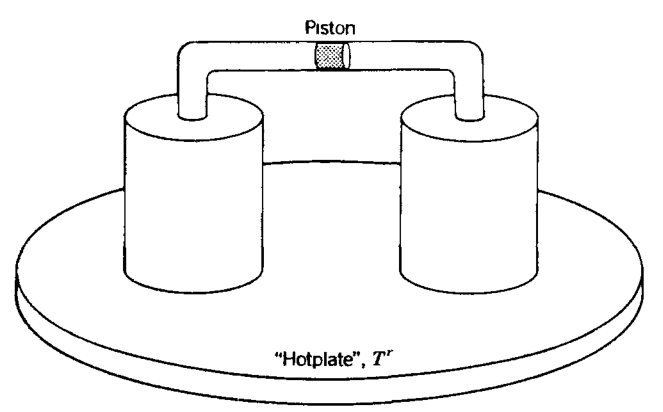
\includegraphics[width=0.6\textwidth]{fig6.1.png}
}

作为Helmholtz势用途的一个例证我们先考虑一个复合系统,这个复合系统由两个被一个可移动的、绝热的、不可透过的壁(例如一个刚性绝热活塞)隔开的简单系统组成。
这两个子系统每一个都与温度$T^r$的热库之间有热接触。
问题是预测两个子系统的体积$V^{(1)}$和$V^{(2)}$。
我们有
\begin{equation}
\label{equ6.23}
P^{(1)}\left(T^r, V^{(1)}, N_1^{(1)}, N_2^{(1)}, ...\right)=P^{(2)}\left(T^r, V^{(2)}, N_1^{(2)}, N_2^{(2)}, ...\right)
\end{equation}
这是一个包含两个变量$V^{(1)}$和$V^{(2)}$的方程;所有其余量都是常数。封闭条件
\begin{equation}
\label{equ6.24}
V^{(1)}+V^{(2)}=V
\end{equation}
提供了另一个需要的方程,使得$V^{(1)}$与$V^{(2)}$可以被明确解出。

在能量表象中我们亦能发现压强相等,正如在方程$6.23$中那样,但此时压强是熵、体积、摩尔数的函数。
我们将需要状态方程来把熵同温度与体积联系在一起;$6.23$与$6.24$两个同时存在的方程将变成$4$个。

尽管这种从$4$个方程到$2$个的简化也许看起来仅仅是个微小的成功,在更加复杂的情形下这种简化将带来巨大的方便。
也许关于这个概念的更加大价值是Helmholtz表象让我们将我们的思考过程没有干扰地集中在我们感兴趣的子系统上,与此同时只把热库视为一个隐含的角色。
最后,由于数学技巧上的原因(这将在第$16$章中详细讲到),在Helmholtz表象下统计力学的计算将被巨大地简化,使得难以对付的计算成为可能。

对于一个与热库有接触的系统,Helmholtz势可以被解释为一定温度下可获得的功。考虑一个与热库有热接触的系统,它与一个可逆功源(reversible work source)之间有相互作用。在一个可逆过程中给可逆功源(reversible work source)输入的功与系统减少的能量相等,并且
\begin{align}
\label{equ6.25}
dW_{RWS}&=-dU-dU'=-dU-T^rdS^r \\
\label{equ6.26}
                  &=-dU+T^rdS=-d(U-T^rS) \\
\label{equ6.27}
                  &=-dF
\end{align}
因此在一个可逆过程中一个与热库有接触的系统所释放的能量与这个系统Helmholtz势减少的量相等。
Helmholtz势经常被称作Helmholtz自由能,尽管短语“一定温度下可获得的功”更不容易被误解。

\subsection*{例子1}
一个圆筒内部包含一个活塞,活塞的每一侧都有一摩尔的单原子分子理想气体。
圆筒的壁是透热的,整个系统浸入到一个温度在$0$摄氏度的大液浴(一个热库)中。
这两个气体子系统(活塞的两边)的初始体积分别为$10$升和$1$升。
活塞现在被可逆地移动,使得其两边最后的体积分别为$6$升和$5$升。
问做了多少功?
\subsubsection*{答案}
正如在问题$5.3-1$中读者见到的那样,Helmholtz势表象中单原子分子理想气体的基本方程式为
\begin{equation}
\notag
F=NRT\left\{\frac{F_0}{N_0RT_0}-ln\left[\left(\frac{T}{T_0}\right)^{3/2}\frac{V}{V_0}\left(\frac{N}{N_0}\right)\right]\right\}
\end{equation}
当$T$与$N$为常数时这意味着
\begin{equation}
\notag
F=常数-NRTlnV
\end{equation}
Helmholtz势的变化为
\begin{equation}
\notag
\Delta F=-NRT[ln6+ln5-ln10-ln1]=-NRTln3=-2.5kJ
\end{equation}
因此$2.5kJ$的功被用于这个过程。

在这里注意到一件有趣的事情,所有的能量都来自于热库。
单原子分子理想气体的能量仅仅是$\frac{3}{2}NRT$,因此它在一定的温度下是个常数。
然而,我们从热库中吸取能量并将它作为注入到可逆功源的功的事实并不违反Carnot效率原理,因为气体子系统并不处在它们的初始态上。
除了这些子系统的能量保持恒定的事实外,它们的熵增加了。
{
    \centering
    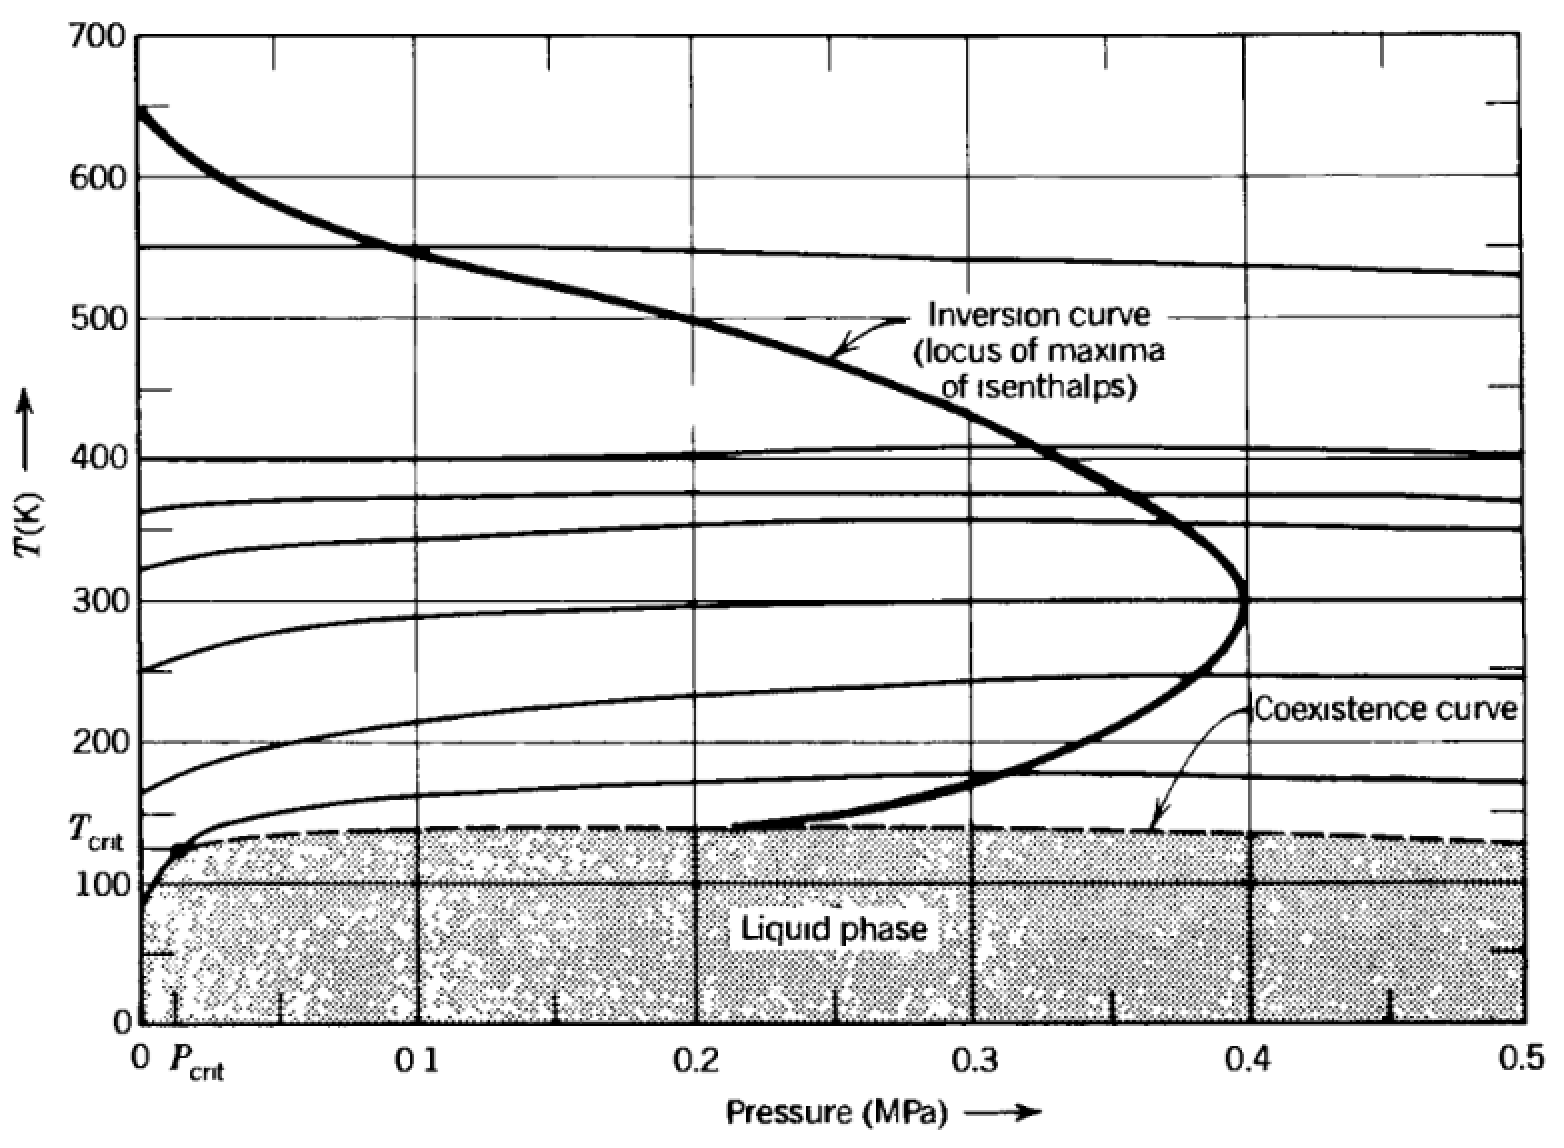
\includegraphics[width = .8\textwidth]{fig6.4.png}
    \figcaption{氮气的等焓线(实线),温度转换曲线(粗实线),以及气液共存线。半定量的图。}\label{fig6.4}
}

氮气的等焓线如图\ref{fig6.4}所示,是有顶点的上凸曲线。如果初始温度和压强再这些顶点的左侧,则节流过程将会冷却气体。如果在右侧则压强的微弱减小会加热气体(当然如果有巨大的压强差越过顶点的话就可以冷却或者加热气体)。等焓线的顶点因此就决定了转换曲线,在顶点上小的压强变化不会加热或者冷却气体。%\mpar{此曲线的得出依靠计算Joule-Thomson系数的$0$点连接起来而绘制出来,而Joule-Thomson系数为$\alpha=\left(\dfrac{\partial T}{\partial p}\right)_H$。可以看出转换曲线与等焓线的交点都是等焓线上的斜率为$0$的点。}

图\ref{fig6.4}的粗实线就是温度转换曲线,吧等焓线的顶点连接起来就行。图中还有气液平衡态的曲线。曲线下的点是液相,上面是气相。共存曲线的端点为“临界点”,在其附近“气体”和“液体”是无法分辨的,其中细节我们在第\ref{chap9}章讲述。

如果节流过程中压强的改变足够小,我们可以用常规的微分来处理
\begin{align}\label{equ6.38}
dT=\left(\frac{\partial T}{\partial P}\right)_{H, N_1, N_2}dP
\end{align}
其可以用标准的测量值($c_P, \alpha, \kappa_T$)的复杂形式表示出来,我们在第\ref{chap7}章会真的写成那种形式。现在呢可以利用数学恒等式\eqref{equA.22}
\begin{align}\label{equ6.39}
dT=-\left[\left(\frac{\partial H}{\partial P}\right)_T/\left(\frac{\partial H}{\partial T}\right)_P\right]dP
\end{align}
其中省略了下标$N_1, N_2,\cdots$,而摩尔数保持不变。然而,$dH=TdS+VdP$是常数,因此
\begin{align}\label{equ6.40}
dT=-\frac{T(\partial S/\partial P)_T+V}{T(\partial S/\partial T)_P}dP
\end{align}
分母部分是$Nc_P$,类比\eqref{equ3.62}或者\eqref{equ3.65}的“Maxwell关系”得到偏微分$(\partial S/\partial P)_T$等于$(-\partial V/\partial T)_P$(在这里利用的是Gibbs势的亮哥交叉导数)。考虑到$(\partial S/\partial P)_T=-(\partial V/\partial T)_P=-V\alpha$(即\eqref{equ3.67})我们终于得到
\begin{align}\label{equ6.41}
dT=\frac{v}{c_P}(T\alpha-1)dP
\end{align}
这是Joule-Thomson效应的基本方程。当压强变化$dP$为负数的时候,$dT$的符号与括号里面的相反。如果$T\alpha>1$,压强的变化(在“节流过程”中)会冷却气体。反转温度就取决于
\begin{align}\label{equ6.42}
\alpha T_{\text{反转}} = 1
\end{align}

对于理想气体的话热扩散系数$\alpha$等于$1/T$,因此Joule-Thomson过程中没有温度变化。所有的气体在高温和低/中压下都表现的像理想气体,其等焓线变得很“平”,如图\ref{fig6.4}。真是气体在转变温度上下的升温降温过程我们可以从例子2中看到,并由此来估计转变温度。

\subsection*{例子2}
计算正常的气体的转变温度,假定用van der Waals方程\eqref{equ3.41}来描述
\subsection*{答案}
我们首先必须要计算扩散系数$\alpha$。把van der Waals方程\eqref{equ3.41}对$T$在$P$不变下作微分
\[\alpha = \frac{1}{v}\left(\frac{\partial v}{\partial T}\right)_P=\left[\frac{Tv}{v-b}-\frac{2a(v-b)}{Rv^2}\right]^{-1} \]
把等式右边写成$T$和$P$的函数是不现实的。一个近似的做法是考虑到摩尔体积是在$0.02m^3$这个量级的,因此$b/v$的量级为$10^{-3}$而$a/RTv$则在$10^{-3}-10^{-4}$量级(见表3.1)。因此只保留最低级数的$b/v$和$a/RTv$就可以了。令
\[\epsilon_1\equiv\frac{b}{v}\quad \epsilon_2\equiv\frac{a}{RTv} \]
从而
\[\begin{split}
\alpha&=\left[\frac{T}{1-\epsilon_1}-\frac{2T}{v}(v-b)\epsilon_2\right]^{-1}\\
&=\frac{1}{T}\left[\frac{1}{1-\epsilon_1}-2(1-\epsilon_1)\epsilon_2\right]^{-1}
\end{split} \]
而再利用\eqref{equ6.41}
\[dT=\frac{v}{c_P}(T\alpha-1)dP \]
而同时有
\[T_{\text{反转}}\alpha=1 \]
我们从而得到转变温度时
\[[1-\epsilon_1+2\epsilon_2+\cdots]=1 \]
或者说
\[\epsilon_1=2\epsilon_2 \]
反转温度即为
\[T_{\text{反转}}\simeq\frac{2a}{bR} \]
气体在$T_{\text{反转}}$之下则被制冷,之上则被加热。从表3.1中,我们可以计算一些气体的反转温度:$T_{\text{反转}}(\mathrm{H})_2=224$K,$T_{\text{反转}}(\mathrm{Ne})=302$K,$T_{\text{反转}}(\mathrm{N})_2=850$K,$T_{\text{反转}}(\mathrm{O})_2=1020$K,$T_{\text{反转}}(\mathrm{CO})_2=2260$K。经验上来看,反转温度与压强息息相关——在我们这里的计算中那些被忽略的高阶项们。H$_2$的零压反转温度为$204$K,而氖则是$228$K——这与我们的粗犷的计算是符合的相当好的。对于多原子气体就符合的不那么好了,CO$_2$的测量值为$1275$K而我们计算的结果是$2260$K。



\section{Gibbs势;化学反应}
\label{sec6.4}

对于一个与热库和压强库有接触的复合系统,其平衡态使得等温和等压(与库相等)态流形上的Gibbs势最小。

Gibbs势是以自变量为$T, P, N_1, N_2, ...$的自然的函数\mpar{原文:{natural function}},在分析包含恒定$T$和$P$的问题时它尤其方便。
在通常的经验中,无数过程发生于暴露在大气中的系统,因此有恒定的温度和压强。
且有意思的过程常常发生在作为热库和压强库的大系统的一个小的子系统中(就像在大红酒桶中发酵的葡萄一样)。

组分系统的Gibbs势与单一组分的化学势有关,对于$G=U-TS+PV$,将Euler关系式$U=TS-PV+\mu_1N_1+\mu_2N_2+...$代入,我们发现
\begin{equation}
\label{equ6.43}
G=\mu_1N_1+\mu_2N_2+...
\end{equation}
因此,对于一个单一组分系统摩尔Gibbs势可写作$mu$
\begin{equation}
\label{equ6.44}
\frac{G}{N}=\mu
\end{equation}
但对于一个多组分系统
\begin{equation}
\label{equ6.45}
\frac{G}{N}=\mu_1x_1+\mu_2x_2+...+\mu_{r}x_{r}
\end{equation}
此处$x_J$是第$J$个组分的摩尔分数($N_J/N$)。
据此,化学势经常在单一组分系统中被称作\emph{摩尔Gibbs势},在多组分系统中被称作\emph{分摩尔Gibbs势}。

化学反应的热力学就是Gibbs势极为重要的应用。

考虑化学反应
\begin{equation}
\label{equ6.46}
0\rightleftharpoons \sum_{1}^{r}\nu_JA_J
\end{equation}
其中$\nu_J$是章节$2.9$中定义的化学计量系数。
Gibbs势随摩尔数变化$dN_J$的变化为
\begin{equation}
\label{equ6.47}
dG=-SdT+VdP+\sum_J \mu_J dN_J
\end{equation}
然而摩尔数的变化必须与化学计量系数成正比
\begin{equation}
\label{equ6.48}
\frac{dN_1}{\nu_1}=\frac{dN_2}{\nu_2}= \dots \equiv d\tilde{N}
\end{equation}
或者,等价地,
\begin{equation}
\label{equ6.49}
dN_J=\nu_J d\tilde{N}
\end{equation}
其中$d\tilde{N}$仅仅是一个在方程$6.48$中定义的比值因子。
如果化学反应在常温常压(比如开容器)中进行,那么平衡条件表明
\begin{equation}
\label{equ6.50}
dG=d\tilde{N}\sum_{J}\nu_{J}\mu_{J}=0
\end{equation}
或者
\begin{equation}
\label{equ6.51}
\sum_{J}\nu_{J}\mu_{J}=0
\end{equation}

如果每种化学组分的初始量为$N_J^0$,化学反应进行到一定程度时,新的摩尔数
\begin{equation}
\label{equ6.52}
N_J=N_J^0+\int dN_J=N_J^0+\nu_J \Delta\tilde{N}
\end{equation}
其中$\Delta\tilde{N}$是比值因子。
方程$6.51$中的化学势为$T$,$P$和摩尔数的函数,因此是未知参数$\Delta\tilde{N}$的函数。
方程$6.51$的解$\Delta\tilde{N}$决定了复合系统的平衡态。

只有在每种组分的量足够使得其在平衡态到来之前不会被耗尽时这个解才是合适的。
也就是说,方程$6.52$中量$N_J$都不是负的。
这种考虑用名词\emph{反应进度}来表达最方便。

在所有$N_J$都保持正数(方程$6.52$)下$\Delta\tilde{N}$的最大值定义了反应的最大允许程度。
类似地,在所有$N_J$都保持正数(方程$6.52$)下$\Delta\tilde{N}$的最小值定义了逆向反应的最大允许程度。
平衡态下$\Delta\tilde{N}$的实际值可以是这两个极端之间的任何地方。
\emph{反应进度}$\varepsilon$被定义为
\begin{equation}
\label{equ6.53}
\varepsilon \equiv \frac{\Delta\tilde{N}-\Delta\tilde{N}_{min}}{\Delta\tilde{N}_{max}-\Delta\tilde{N}_{min}}
\end{equation}

化学平衡方程$(6.51)$的直接解产生的$\Delta\tilde{N}$也许大于$\Delta\tilde{N}_{max}$或小于$\Delta\tilde{N}_{min}$。
在这种情况下过程由其中一种组分的耗尽决定。
其相关的$\Delta\tilde{N}$值就是$\Delta\tilde{N}_{max}$(或$\Delta\tilde{N}_{min}$)。
尽管$\sum_{J}\nu_{J}\mu_{J}$并不达到$0$,它达到系统所允许的最小绝对值。

尽管分摩尔Gibbs势刻画了平衡条件,焓表达的是\emph{反应热}。这个事实由焓作为恒压下“热流势”(方程$6.29$)的意义而来。
也就是说,系统周围的热流在化学反应中与焓变相等。
焓变反过来又与化学势有关,因为
\begin{equation}
\label{equ6.54}
H=G+TS=G-T\left(\frac{\partial G}{\partial T}\right)_{P, N_1, N_2,}
\end{equation}
如果无限小化学反应$\Delta\tilde{N}$发生了,$H$和$G$都会变并且
\begin{equation}
\label{equ6.55}
dH=\frac{dH}{d\tilde{N}}d\tilde{N}=\frac{dG}{d\tilde{N}}d\tilde{N}-T\frac{\partial}{\partial T}\left(\frac{dG}{d\tilde{N}}\right)_{P, N_1, N_2,}d\tilde{N}
\end{equation}
但是Gibbs函数的变化为
\begin{equation}
\label{equ6.56}
dG=\sum_{1}^{r}\mu_JdN_J=\left(\sum_1^r \nu_J\mu_J \right)d\tilde{N}
\end{equation}
由此可知
\begin{equation}
\label{equ6.57}
\frac{dG}{d\tilde{N}}=\sum_1^r \nu_J\mu_J
\end{equation}
$dH/d\tilde{N}$是\emph{反应热};也就是在平衡态下每单位反应吸收的热。
它在吸热反应下为正,放热反应下为负。

随着平衡态下方程$6.58$中求和的消失,直觉上这个量对于温度的导数与平衡态对温度的依赖有关。
我们会发现只有在理想气体的特殊情况下推导这个关系才是方便可行的,在章节$13.4$中。
然而,注意到这个关系的合理之处并且认识到这种关系允许反应热被不同温度下特定的平衡态而不是相对麻烦的测热实验所测量是相当有趣的。

分析化学反应的广泛方法当运用在特定系统中就会变得特定而确切。
为了决定特定情形下将要进行的处理方法,读者也许会希望此处插入第$13$章——尤其是章节$13.2$,有关理想气体的化学反应。

\subsection*{例子3}
5摩尔的$H_2$,1摩尔\ce{CO2},1摩尔$CH_4$,和3摩尔$H_2O$在一个维持在温度$T_0$和压强$P_0$的容器中反应。
有关反应是
\[ 4H_2+CO_2\leftrightharpoons CH_4+2H_2O \]
由平衡态下的解得到$\Delta \tilde{N}=-\frac{1}{2}$。每种组分的摩尔数是多少?如果压强增加至$P_1$($P_1>P_0$)并且温度保持恒定($=T_0$)平衡态条件给出$\Delta \tilde{N}=1, 2$。每种组分的摩尔数是多少?
\subsubsection*{答案}
我们首先写下每种组分的方程$6.52$:$N_{H_2}=5-4\Delta \tilde{N}$, $N_{CO_2}=1-\Delta \tilde{N}$, $N_{H_2O}=3+2\Delta \tilde{N}$。
将每个摩尔数设定为$0$我们得到$\Delta \tilde{N}$的4个根:$\frac{5}{4}, 1, -1$和$-\frac{3}{2}$。绝对值最小的正根和负根分别为
\[ \Delta \tilde{N}_{max}=1, \Delta \tilde{N}_{min}=-1 \]
这两个$\Delta \tilde{N}$的界限与反应向前进行得太远时\ce{CO2}的耗尽有关,与反应逆向进行得太远时$CH_4$的耗尽有关。

根据方程$6.53$,反应度
\[ \varepsilon=\frac{\Delta \tilde{N}+1}{1+1}=\frac{1}{2}(\Delta \tilde{N}+1) \]
若平衡态条件的解给出$\Delta \tilde{N}=-\frac{1}{2}$那么$\varepsilon=\frac{1}{4}$且$N_{H_2}=3, N_{CO_2}=\frac{3}{2}, N_{CH_4}=\frac{1}{2}$且$N_{H_2O}=2$。

如果增大的压强使得$\Delta \tilde{N}$的解变为$+1, 2$我们去掉在$\Delta \tilde{N}$允许范围以外的值;它将导致不物理的解$\varepsilon=1.1$但是$\varepsilon$必须在$0$和$1$之间,因此反应在$\Delta \tilde{N}=\Delta \tilde{N}_{max}=\frac{1}{2}$(或$\varepsilon=1$)时终结。
最终摩尔数为$N_{H_2}=1, N_{CO_2}=\frac{1}{2}, N_{CH_4}=2, N_{H_2O}=5$。


\section{其它势}
\label{sec6.5}

各种其它势也许会在特定情况下变得很有用。
其中一个应用中可以知道一种广泛的方法。

\subsection*{例子4}
一个体积为$V$的瓶子,内含$N$摩尔的糖,它被水和一个刚性盖子所填满。
这个刚性盖子可以透过水但是不能透过糖。
这个瓶子浸入到一个大的水桶中。
水桶中压强为$P_v$且温度为$T$。
我们要找到瓶子中的压强$P$和摩尔数$N_w$。
\subsubsection*{答案}
假设我们有两组分(糖水混合物)的基本方程。
这个基本方程在表象$U[T, V, \mu_{w}, N_{s}]$下写成;这个表象下$S$和$N_{w}$被它们相应的强度量所取代,但体积$V$和糖的摩尔数$N_{s}$保持不变。
透热壁保证了温度可以被大水桶(热库)所决定,且半透的瓶盖保证了$\mu_{w}$的值由水桶(“水库”)所决定。
没有剩下的问题了!我们知道所有广义势$U[T, V, \mu_{w}, N_{s}]$的独立变量,为了得到瓶子中的压强,我们仅仅需要对势求导:
\[ P=-\frac{\partial U[T, V, \mu_{w}, N_{s}]}{\partial V} \]
将它与能量或熵表象下的解的比较留给读者。
各种未被要求的变量也进入到分析当中——例如瓶中的熵,或桶中的熵,能量,摩尔数。
对于每种外来变量,都需要为消去它增加一个方程。
合适表象的选择很明显是简化问题的关键,并且是热力学计算的实践。


\section{经验数据的编制;生成焓}
\label{sec6.6}

原则上,对于特定系统的热力学数据,通过表格形式列出温度、压力和组成(单个组分的摩尔分数)的吉布斯势函数是最为简洁方便的。
这样的表格以最便于实验工作者的方式呈现基本方程。

实践中,通常编制$h(T,P)$、$s(T,P)$和$v(T,P)$的数据,由此可得摩尔吉布斯势$g=h-Ts$。
$h$、$s$和$v$的列表虽冗长却方便使用。
对于多组分系统,有必要对所有感兴趣的成分进行类似的编辑。

系统两个状态间的摩尔焓之差可以通过数值积分$\rd h=\dbar Q/N+v \rd  P$来实验性评价,其中$\dbar Q$、$P$和$v$可沿积分路径测量得到。


与能量或任何其它热力学势类似,焓的绝对标度可以是任意的,有一个常数的不确定度。
为了编制数据,令标准温度和压力下处于其最稳定形式的各化学元素的摩尔焓为零,由此明确定义焓值。一般
\[ T_0 = 298.15K = 25^{\circ}\qquad P_0 = 0.1 \text{MPa} = 1 \text{atm} \]
由此定义的焓称作\textit{生成焓}。

在生成焓的定义中提及的“最稳定形式”应照此理解:例如,令分子形式($O_2$)而非原子形式($O$)氧的焓值为零,因为分子形式在标准温度和压力下是最稳定的形式。

如果1摩尔碳与1摩尔$O_2$于标准温度和压力下反应生成1摩尔\ce{CO2},便能观察到$393.52\times10^3\text{J}$热量释放。因此标准状态下\ce{CO2}的生成焓表示为$-395.32\times10^3\text{J}/\text{mole}$。
这便是\ce{CO2}的\textit{生成焓}。
任何其他温度或压力下\ce{CO2}的生成焓可由积分$\rd h=\dbar Q/N+v\rd P$得到。
%\dbar Q还是\dbar Q不确定

在JANAF热化学表(Dow Chemical company,Midland, Michigan)和其他各种类似的数据表中,列出了大量化合物的标准生成焓及相应标准状态下的标准摩尔吉布斯势和摩尔熵。

当自变量$T$和$P$的值所属范围很大,列出特定材料的几个性质(比如$h$、$s$和$v$)甚至单个性质都会令热力学性质表变得极其庞大。
然而,对于水这样的普通材料,已有非常丰富的数据表可供查阅,这些表叫做“蒸汽特性表”。
有一种叫做“过热蒸汽表”的表格列出了不同压力下摩尔体积$v$、能量$u$、焓$h$和熵$s$关于温度的函数。
含少量压力值的这种表(由Sonntag和van Wilen制作)的一份摘录列于表6.1。%表格引用
还有一种叫做“饱和蒸汽表”的表格给出了$P$和$T$处于气-液共存曲线时水的液态和气态相的特性值。
这种“饱和蒸汽表”将在表9.1给出。%表格引用

另一种很常见的热力学数据表示方法是“热力学图表”或图示。
这种图表必然牺牲了精度,却简洁紧凑地概括了大量数据。
从概念上,这类最简化的图表以$T$和$P$标识两个坐标轴。
然后,单组分系统以一族恒定吉布斯势$\mu$的曲线表示。
原则上,所有想要的数据都能依此评估。
比如,测定摩尔体积就需要读取相应温度下附近两点的压力值,由此得到微分$\left(\Delta\mu/\Delta P\right)_T$的数值估计,即摩尔体积。
替代性地,图上覆盖着一族等体积线,每个等体积线标着一个$v$。
类似地,恒定摩尔熵$s$、恒定摩尔焓$h$、恒定摩尔热膨胀系数$\alpha$、恒定值$\kappa$等都覆盖在上面。
唯一的限制是图表的可读性。

不难发现,用笛卡尔坐标表示变量毫无独特之处。
每一族曲线作为一个(曲线)坐标系。
因此,在相应等体积线和绝热线的交叉处可以定位到给定$v$和$s$的点,然后就能读取其他图中变量的值。

实际使用中有各式各样的热力学图表。
一种流行的表叫做Mollier表——它将摩尔焓$h$和摩尔熵$s$作为笛卡尔坐标,同时将等体积线和等压线覆盖其上。
还有一种常用图表(一种“温度——熵值”表)将温度和熵值作笛卡尔坐标同时覆以摩尔焓$h$及其他热力学函数,限制数量的主要是可读性。(图6.5)%图片引用

只有少量成分相对简单的系统有这样全的热力学数据。
对于大多数系统只有部分数据可获取。
一个大规模的数据编制项目已经存在。
\textit{International Journal of Thermophysics}(lenum Press, New York and London)提供当前热物理学的测量报告。
坐落于普渡大学的信息和数值分析与编纂中心(“CINDAS”)出版一系列的数据收集资料,其中值得注意的是\textit{Thermophysical Properties Reaserch Literature Retrieval Guide: 1900-1980}(七卷),由J. F. Chancy 和 V. Ramdas(Plenum Publishing Corp., New Yoor, 1982)编辑。

最后,简单回顾一下通过最少的表格所列或测量得到的数据构造单组分系统的基本方程的过程。
所需最少信息为$\alpha(T,P)$、$c_p(T,P)$和$\kappa(T,P)$,加上参考状态(可能是信息焓)的$v_0$和$s_0$值。
由这些数据可以通过对Gibbs-Duhem关系式$\rd \left(G/N\right)=-s\rd T+v\text{P}$积分得到摩尔吉布斯势——前提是由以下方程得到$s(T,P)$和$v(T,P)$的数值积分
\[\rd s=\left(\frac{\partial s}{\partial T}\right)_P\rd T+\left(\frac{\partial s}{\partial P}\right)_T\rd P=\frac{c_P}{T}\rd T-v\alpha\rd P\]
和
\[\rd v=v\alpha\rd T-v\kappa_T\text{P}\]

这些积分都必须遍及整个$T-P$平面的路径网——常常是一项巨大的数值工作。

\section{Massieu函数的最大值原则}
\label{sec6.7}
在能量表示中,熵值为常量时能量为最小值。由此可见在(加强的)变量变换后为常值时能量的Legendre表相变换为最小值。
类似地,在熵表示中,能量为常量时熵为最大值。同理可知在(加强的)变量变换后为常值时熵的Legendre表相变换为最大值。%intensive 作何翻译

对于三个常见的Massieu函数中的两个,最大值原理可以简单得到,因为这些函数直接与势能相关(比如,能量的变换)。
从\eqref{equ5.61},得到
\begin{equation}
S\left[\frac{1}{T}\right]=-\frac{F}{T}
\end{equation}
并且,既然$F$在温度恒定时为最小值,$S[1/T]$显然是最大值。再一次,由\eqref{equ5.63}
\begin{equation}
S\left[\frac{1}{T},\frac{P}{T}\right]=-\frac{G}{T}
\end{equation}
进一步可见,既然$G$在恒温恒压下是最小值,$S[1/T,1/P]$显然是最大值。

至于剩下的那个常见的Massieu函数$S[P/T]$,可以重复\ref{sec6.1}的逻辑。
现在关注一个与保持$P/T$为常值但允许$1/T$变化的热库相接触的系统。
既然已经意识到这样一个热库是数学上的虚构而非物理上可行的装置,那么相应的$S[P/T]$的最值原则也是子虚乌有了。
然而沿着\ref{sec6.1}这条线一路导出这个定理这一过程对于好奇的读者来说不失为一个有趣的练习。
